\chapter{Evaluation of the Best Classification Method}
\label{chapter_classification}
\section{Considered classification methods}
\label{sec_considered_classif}
The goal of our analysis is to classify $y \in \left\lbrace female, male \right\rbrace $ given the data matrix $\mat{X}$ of our 17 predictors. 
We are interested in determining not only the model with the best predictive performance, but also the most significant features of human voice. 
We argue that sensitivity and specificity are of equal importance in our setting and, thus, our objective is to minimize total misclassification error. 
Also we note that our classes our perfectly balanced (50/50), so we use a threshold of 0.5 for our Bayes plug-in estimator.
In our analysis we implement the following statistical learning methods to predict the class of $ y \in \left\lbrace female, male \right\rbrace$.
\begin{itemize}
	\item \textbf{Logistic Regression:} models the posterior probability of response $y\in \left\lbrace female, male \right\rbrace$, given the predictors $\mat{X}$, using the logistic function;
	
	\item \textbf{Regularized Logistic Regression:} The $\ell_1$-penalty~(LASSO) can be used for variable selection and shrinkage with logistic regression. 
	It is a useful approach to examine which features are  important in voice analysis;
	
	\item \textbf{Linear Discriminant Analysis (LDA):} LDA makes the assumption that the conditional densities $f \left(\mat{X}|y=male \right)$ and $ f \left(\mat{X}|y=female \right)$ are both multivariate Gaussian with a common covariance matrix. 
	It belongs to a family of techniques that use linear boundaries to separate classes in classification problems. 
	If the assumption of normality is realistic, then LDA is expected to provide better results than logistic regression;
	
	\item \textbf{Quadratic Discriminant Analysis (QDA):} QDA is a similar method to LDA. 
	The multivariate normality assumption remains, but unlike LDA, QDA assumes that each class has its own covariance matrix. 
	If QDA has better predictive performance than LDA, it is an indication that a linear boundary is not the optimal to separate the 2 classes.
	
	\item \textbf{k-Nearest Neighbors (kNN):} kNN is a non-parametric approach which is highly flexible and uses non-linear decision boundaries. 
	Before the implementation of kNN, it is crucial to scale the data, since this method relies on the euclidean distance between observations;
	
	\item \textbf{Classifications Trees:} Classification trees stratify the feature space recursively into simple regions and assign the label female or male using the majority vote. 
	Bagging, random forests and gradient tree boosting are also implemented with the aim of improving predictive performance;
	
	\item \textbf{Support Vector Machines (SVM):} SVM perform well in classification problems where there is a clear margin of separation. 
	We experiment with 2 kernels: the linear and the radial basis function~(RBF).
\end{itemize}
For an exhaustive description of the classification methods, please refer to~\cite{ESL_2001}.
\section{Classification based on the fundamental frequency}
\label{sec_intuitive_approach}
Based on the exploratory data analysis described in Chapter~\ref{chapter_data_exploration}, we propose to perform the classification based on the ``meanfun'' feature alone. 
This will give a baseline for further analysis described in the remaining of this Chapter.

To perform the analysis, we randomly split the dataset into a training set~( \SI{80}{\percent}) and a test set~(\SI{20}{\percent}). 
The training set is used to fit the models and for best parameter selection if needed. The test set is used to compute the classification error and to compare the models. The classification error considered in the study is the $0-1$ loss. 
The experiments have been performed on Python \num{3}\footnote{\url{{https://github.com/AdriBesson/Statistical_learning_course/tree/develop/project}}} with a single seed number for reproducibility of the results.
\begin{table}[htb]
	\ra{1.2}
	\caption{Classification Error Estimate of the Methods for Classification With ``meanfun'' Feature}
	\begin{center}
		\begin{tabular}{@{} c c c @{}}\toprule
			Type & Methods & \\
			\midrule
			\multirow{5}{*}{Max. Likelihood} & Logistic reg. & \num{0.0536} \\
			& Logistic reg. - Ridge & \num{0.0505}  \\
			& LDA & \textbf{\num{0.0489}} \\
			& QDA & \textbf{\num{0.0489}} \\
			\cmidrule{1-3}
			\multirow{3}{*}{Trees} & Tree & \num{0.0505} \\
			& Bagging & \num{0.0505} \\
			& XGBoost & \num{0.0505}\\
			\cmidrule{1-3}
			\multirow{2}{*}{SVM} & Linear & \num{0.0505} \\
			& Gaussian & \textbf{\num{0.0489}} \\
			\cmidrule{1-3}
			x & kNN & \num{0.0520}\\
			\bottomrule
		\end{tabular}
	\end{center}
	\label{tab_res_meanfun}
\end{table}

The results, summarized in Table~\ref{tab_res_meanfun}, show that the classification error is already very low when considering only the ``meafun'' feature. Indeed the average classsification error of the different classifiers is \num{0.0509}. Thus, ``meafun'' is a very good feature for classification which is in accordance with the exploratory data analysis described in Chapter~\ref{chapter_data_exploration}. 

Regarding the classifiers, it can be seen that some of the ones described in Section~PUTREF, are not mentioned in Tabel~\ref{tab_res_meanfun}. Indeed, they do not make sense when considering only one feature for classification. 
About the relative performance of the different classifiers, the results are homogeneous around the average classification error and all the classifiers perform well. Zero-order methods such as tree-based methods (with one predictor, tree-based methods are nothing else than a threshold) already give a low classification error. More sophisticated methods, such as linear methods or kernel SVM, give results very similar to or slightly better than zero-order methods.

\section{Classification based on a $80/20$ split of the dataset}
\label{sec_naive_strat}

\subsection{Experimental settings}
To perform the analysis, we randomly split the dataset into a training set~( \SI{80}{\percent}) and a test set~(\SI{20}{\percent}). 
The training set is used to fit the models and for best parameter selection if needed. 
he test set is used to compute the classification error and to compare the models. The classification error considered in the study is the $0-1$ loss. 

The models compared in the study are the ones described in Section~\ref{sec_considered_classif}. 
The errors are computed for \num{5} seed numbers in order to study the variability of the models with respect to the training/test sets and their initialization. 
The results are reported in Table~\ref{tab_res_naive}.

\begin{table}[htb]
	\ra{1.2}
	\caption{Classification Error Estimate of the Methods for Different Seed Numbers With $80/20$ Split}
	\begin{center}
		\begin{tabular}{@{} c c c  c c c c c c @{}}\toprule
			\multirow{2}{*}{Type} & \multirow{2}{*}{Methods} &  \multicolumn{5}{c}{Seed number}
			& 	\multirow{2}{*}{Mean} & \multirow{2}{*}{Std.} \\
			& & 1 & 2 & 3 & 4 & 5 & & \\
			\midrule
			\multirow{5}{*}{Max. Lik.} & Log. reg. & \num{0.0158} & \num{0.0347} & \num{0.0315} & \num{0.0237} & \num{0.0221} & \num{0.0256} & \num{0.00760} \\
			& Log. reg. - $\ell_2$ & \num{0.0158} & \num{0.0315} & \num{0.0315} & \num{0.0189} & \num{0.0284} & \num{0.0252} & \num{0.00740}\\
			& Log. reg. - $\ell_1$ & \num{0.0315} & \num{0.0363} & \num{0.0379} & \num{0.0284} & \num{0.0300} & \num{0.0328} & \num{0.00408}\\
			& LDA & \num{0.0315} & \num{0.0410} & \num{0.0379} & \num{0.0284} & \num{0.0268} & \num{0.0331} & \num{0.00611}\\
			& QDA & \num{0.0347} & \num{0.0347} & \num{0.0347} & \num{0.0268} & \num{0.0363} & \num{0.0334} & \num{0.00377}\\
			\cmidrule{1-9}
			\multirow{5}{*}{Trees} & Tree & \num{0.0379} & \num{0.0426} & \num{0.0315} & \num{0.0284} & \num{0.0300} &  \num{0.0341} & \num{0.00596}\\
			& Pruned Tree & \num{0.0394} & \num{0.0473} & \num{0.0347} & \num{0.0363} & \num{0.0300} & \num{0.0375} & \num{0.00645}\\  
			& Bagging & \num{0.0237} & \num{0.0410} & \num{0.0142} & \textbf{\num{0.0174}} & \num{0.0284} & \num{0.0249} & \num{0.0106}\\
			& Random Forest & \num{0.0189} & \num{0.0347} & \textbf{\num{0.0126}} & \num{0.0205} & \num{0.0205} & \num{0.0215}  & \num{0.00809}\\
			& XGBoost & \num{0.0189} & \textbf{\num{0.0268}} & \textbf{\num{0.0126}} & \num{0.0205} & \textbf{\num{0.0189}} & \textbf{\num{0.0196}}  & \num{0.00506}\\
			\cmidrule{1-9}
			\multirow{2}{*}{SVM} & Linear & \textbf{\num{0.0142}} & \num{0.0315} & \num{0.0284} & \num{0.0189} & \num{0.0252} & \num{0.0237}  & \num{0.00705}\\
			& Gaussian & \num{0.0205} & \num{0.0284} & \num{0.0126} & \num{0.0189} & \num{0.0221} & \num{0.0199} & \num{0.00575}\\
			\cmidrule{1-9}
			x & kNN & \num{0.0300} & \num{0.0347} & \num{0.0252} & \num{0.0379} & \num{0.0300}& \num{0.0315}  & \num{0.00486} \\
			\bottomrule
			\end{tabular}
			\end{center}
			\label{tab_res_naive}
\end{table}

\subsection{Maximum-likelihood methods}
\paragraph{Logistic Regression}
If we run logistic regression on our \num{17} features, we obtain an error rate of 0.0158. The reported p-values indicate that, at \SI{5}{\percent} significance level, the coefficients of the following features are significantly non-zero: ``Q25'', ``Q75'', ``sp.ent'', ``sfm'', ``meanfun'' and ``minfun''. We observe that the lowest p-value corresponds to meanfun, which shows the importance of this particular feature in voice analysis.

\paragraph{Regularized Logistic Regression}
We observe that Ridge regularization gives the same results as logistic regression. However, Lasso regularization performs worse providing a test error of \num{0.0315}. Lasso shrinks the coefficients of 9 predictors to zero, letting only non-zero the following ones: ``Q25'', ``Q75'', ``skew'', ``sfm'', ``mode'', ``minfun'', ``maxfun''. The largest coefficient corresponds to ``meanfun'', confirming its significance.
$$ Plots ~ of ~ parameter~skrinkage$$ 

\paragraph{Linear Discriminant Analysis}
LDA gives a test error of \num{0.0315}. In order to check whether the model assumptions are actually satisfied, we resort to Mardias' test\footnote{\url{https://cran.r-project.org/web/packages/MVN/index.html}} for multivariate normality. Mardias' test is based on the multivariate extensions of skewness and kurtosis measures. Under the null hypothesis, our sample is drawn from a multivariate normal. 
We run Mardias' test on the two data matrices corresponding to male and female classes and conclude that normality assumption is violated. However, the two covariance matrices are quite similar and one can argue that the assumption of a common covariance matrix is realistic. 
To sum up, LDA seems to perform well, despite the lack of normality. We suspect that the reason lies in some particularity of our data set.


\paragraph{Quadratic Discriminant Analysis}
As we have seen above, the two covariance matrices of our two classes (male/female) are indeed close. Hence we expect QDA to perform worse than LDA. Indeed, its performance is slightly worse reporting a test error rate of \num{0.035}.


\subsection{k-Nearest Neighbors}
We use \num{10}-fold cross validation with one-standard-error rule to find that the optimal value for parameter k, is $k=9$. Then we implement \num{9}-NN, which yields a test error of \num{0.03}. We observe a slight improvement compared to LDA and QDA, which can be attributed to the high flexibility of kNN. We reckon that the linear boundary is not the most appropriate to separate the \num{2} classes.
$$ Plot ~ for ~ determing ~ k ~ with ~ CV~ one-standard-error rule $$ 

\settoheight{\BoxPlotFigHeight}{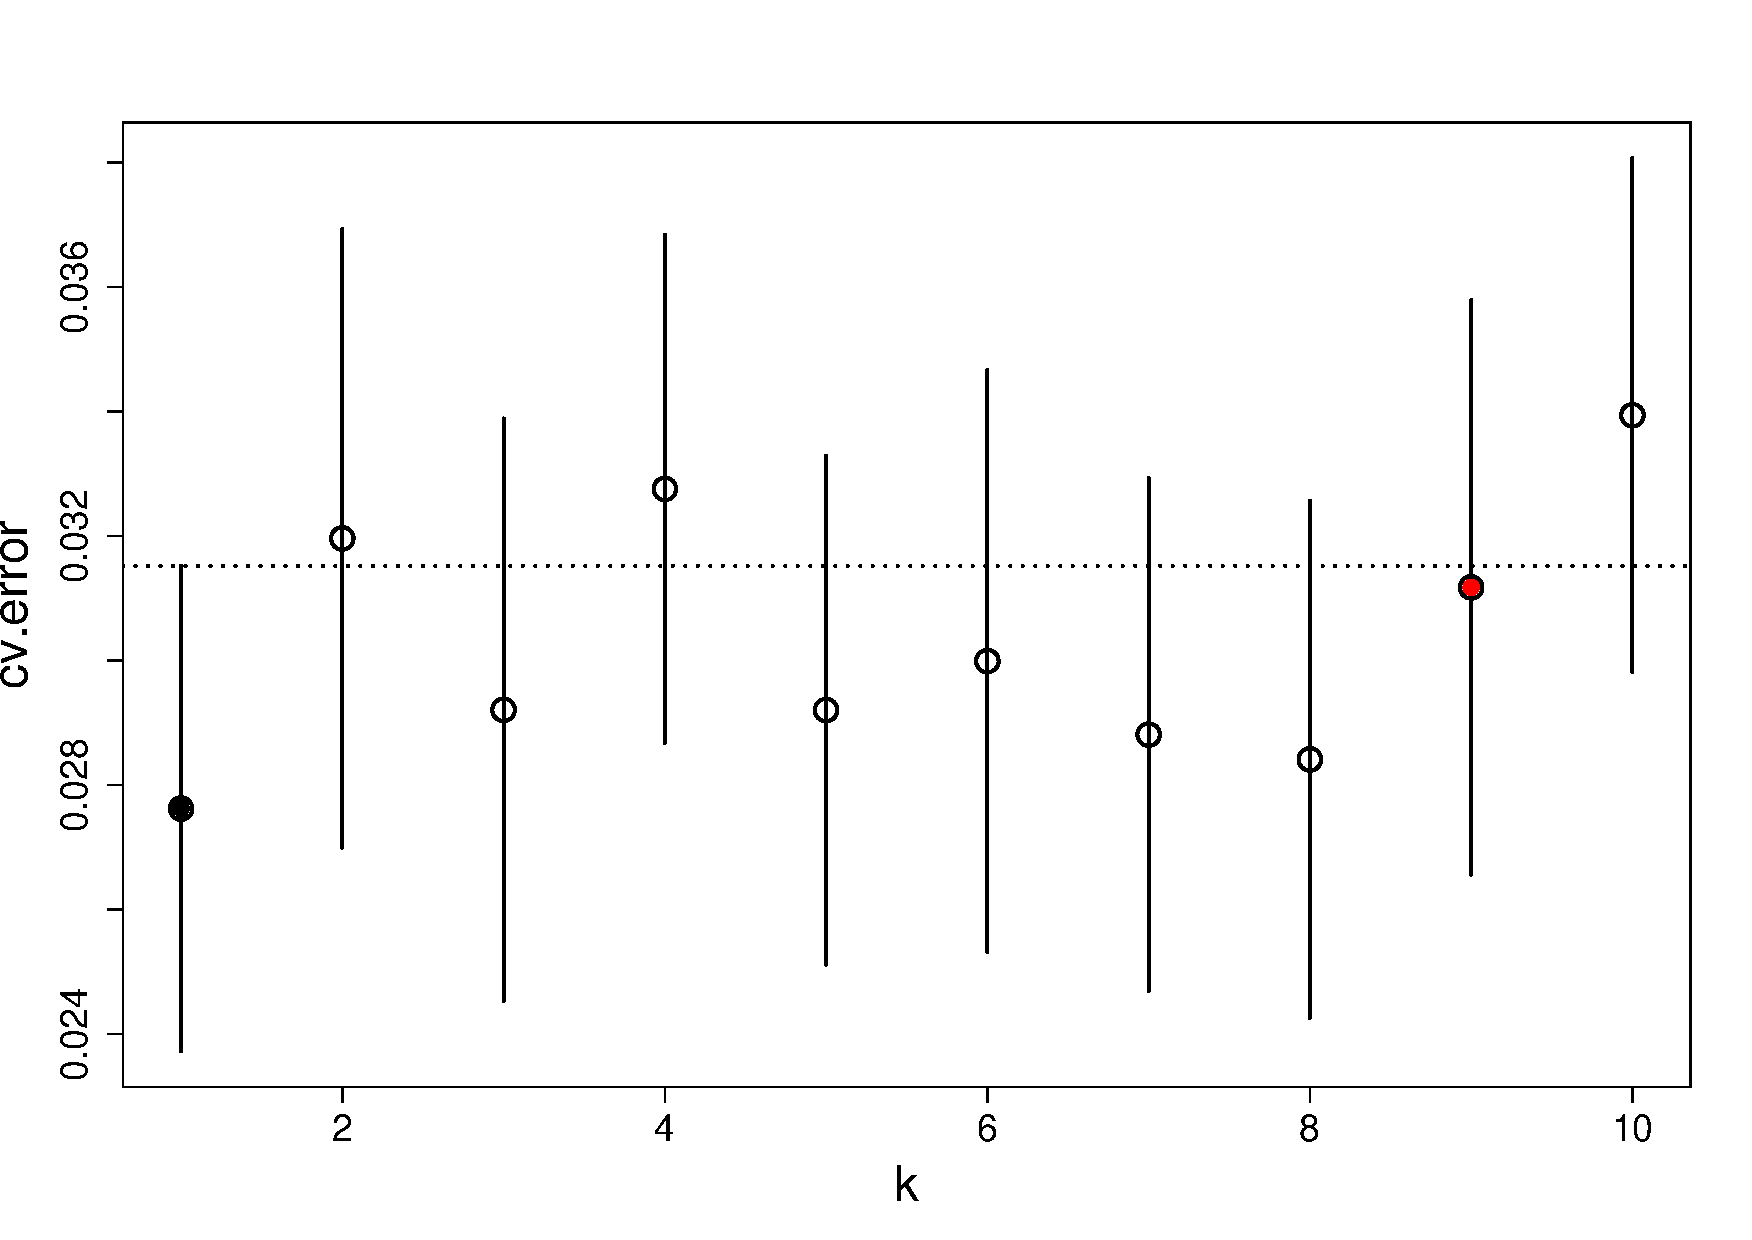
\includegraphics[width=\BoxPlotFigWidth]{figures/Rplot02.pdf}}
\begin{figure}[htb]
	% Maximum length
	\hfill%
	\subcaptionbox{\label{}}{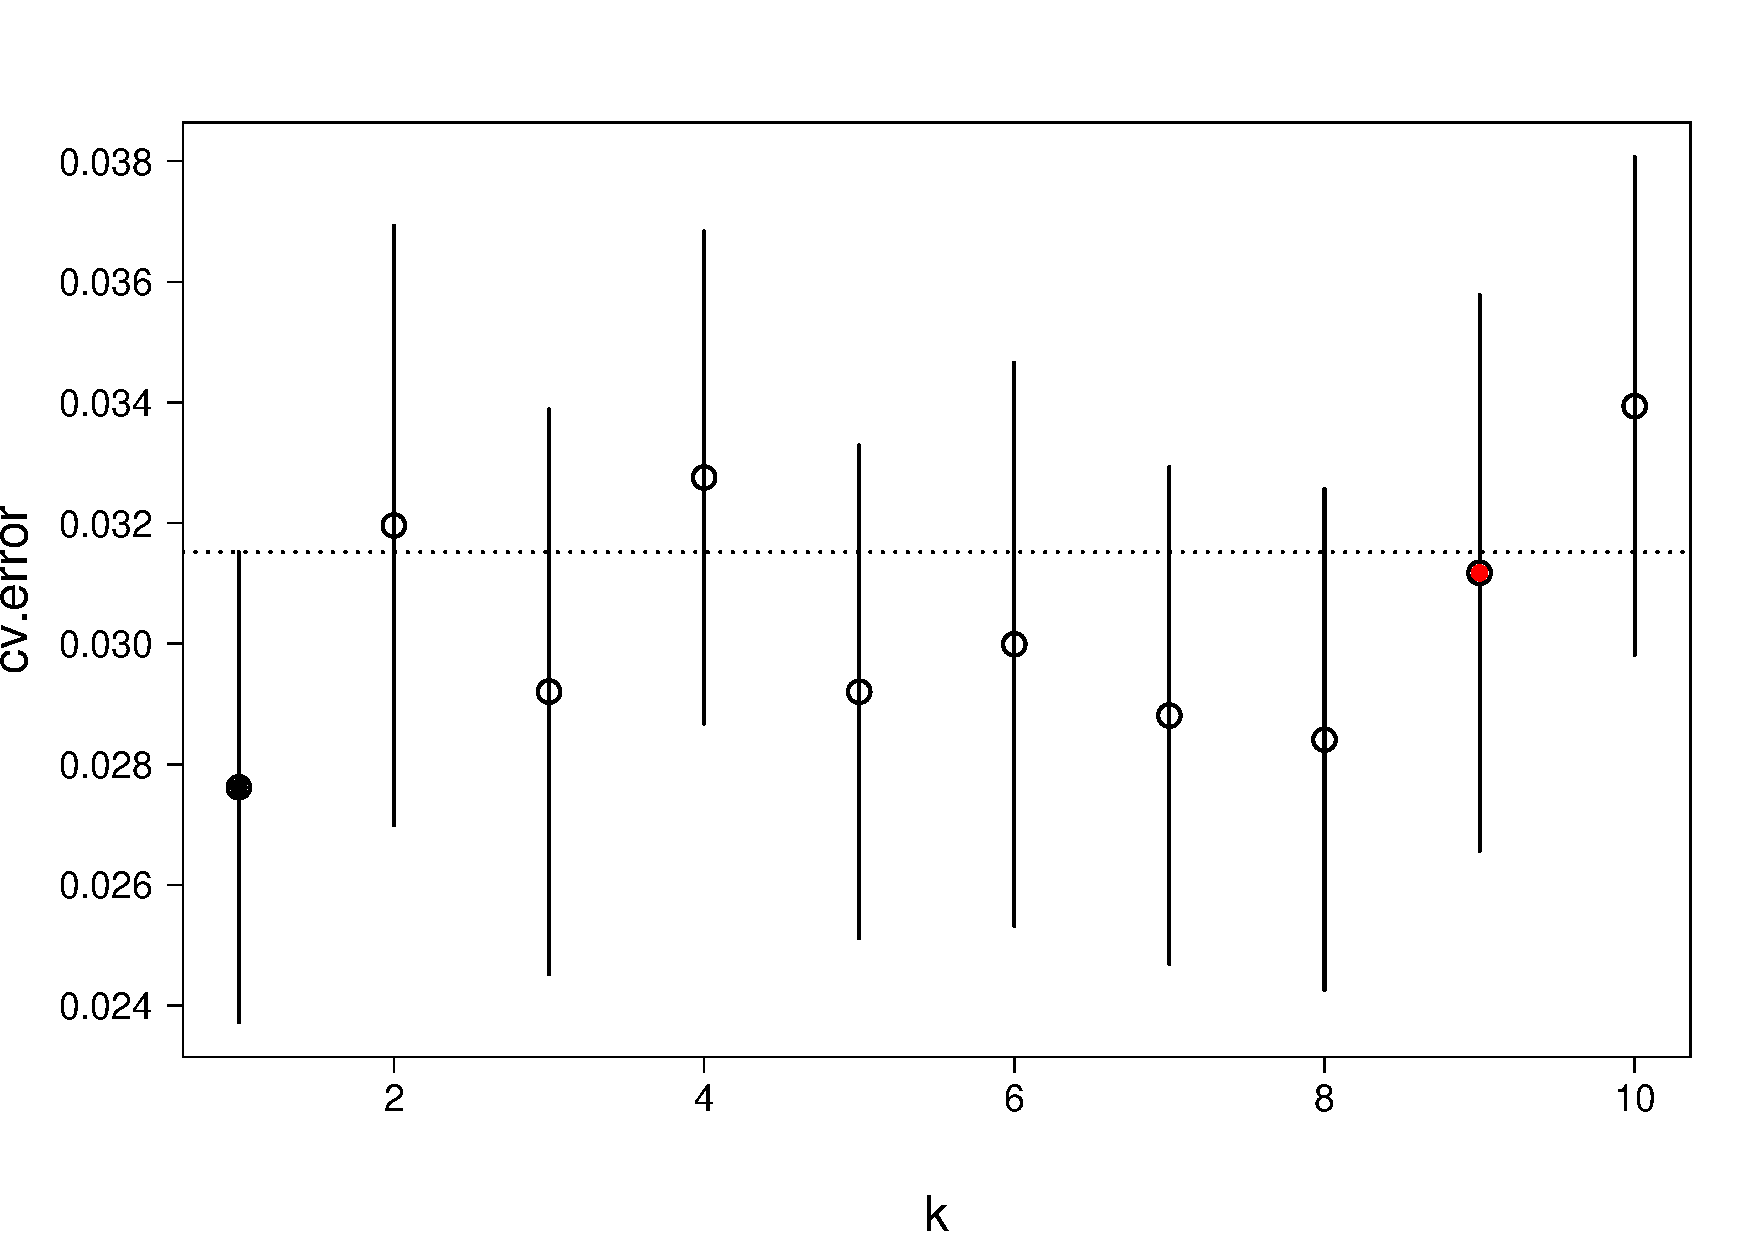
\includegraphics[height=\BoxPlotFigHeight]{figures/Rplot03.pdf}}\hfill%
	\subcaptionbox{\label{}}{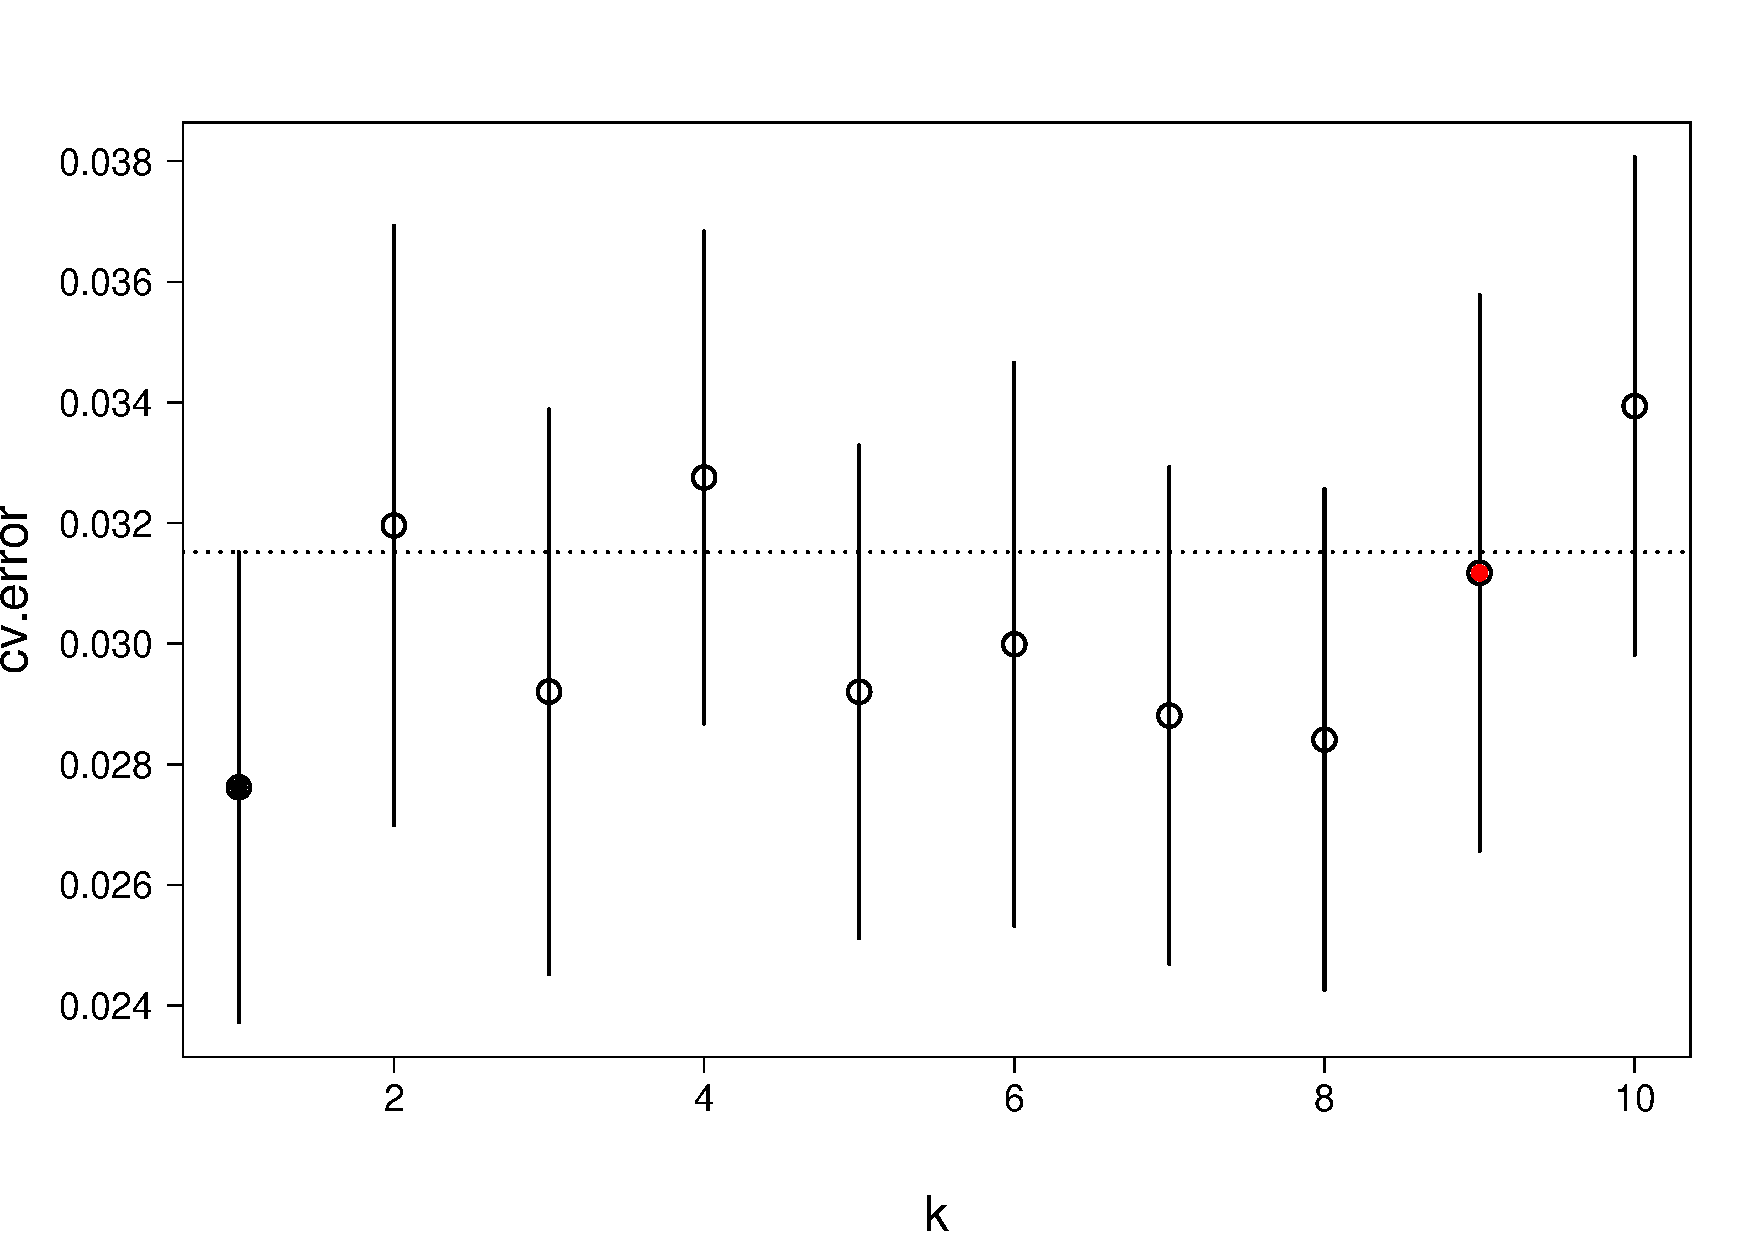
\includegraphics[height=\BoxPlotFigHeight]{figures/Rplot03.pdf}}\hfill\null%
	\caption{}
	\label{fig_test}
\end{figure}

\subsection{Tree-based methods}

\paragraph{Classification Trees}
We begin with fitting a large unpruned tree to our data. We use the cross-entropy impurity measure to grow our tree and obtain a test error of \num{0.038}. Although its predictive performance is quite good in our case, its high complexity prevents it from being interpretable.

$$ Plot ~ of ~ the ~ ugly ~ large ~tree$$


After fitting a large tree, it is sensible to prune it in order to improve its interpret-ability and avoid overfitting. We prune our tree using \num{10}-fold cross validation to determine the cost-complexity parameter, and misclassification error as the loss function. Although the test error has slightly increased, the pruned tree can now be used to convey meaningful results. We also observe that ``meanfun'' is used in the first node, confirming, for one more time, its integral role.

$$ Plot ~ of ~ the ~ pruned~ tree$$

\paragraph{Bagging}
Unpruned trees have low bias but suffer from high variance. Bagging can substantially reduce the variance of unstable procedures like trees, and improve predictive performance. Bagging indeed improves accuracy of our trees, since we obtain a test error of \num{0.0237}. We also stress the importance of Out-of-Bag error estimate, which, in our case, is quite close to the test error.

$$ Plot ~ of ~ OOB~error~ estimate$$ 

\paragraph{Random Forests}
We proceed our analysis with running a random forest. We are particularly interested in this method, since random forests provide measures of variable importance. Mean decrease accuracy and mean decrease gini metrics indicate that ``meanfun'' is the most influential feature, followed by ``Q25''. The test error is \num{0.0189}, which confirms the superb predictive performance of random forests. Again, Out-of-Bag error estimate gives an accurate estimate of test error.

$$ Plot ~ of ~ OOB~error~ estimate$$ 

Partial dependence plots are useful to interpret variable importance in complex ``black box'' methods, such as random forests. These plots illustrate the marginal effect of the selected feature after integrating out the other features. Below we present the partial dependence plot on ``meanfun''. The shape of the curve indicates that the fitted random forest uses a clear threshold that separate the two classes (female/male). Consequently, we can argue that the steepness of the curve in the middle pinpoints the importance of ``meanfun''. 

$$ Plot ~ of ~ partial~dependence$$

\paragraph{Gradient Tree Boosting}
In our quest of determining the model with the best accuracy, we then implement gradient tree boosting by using XGBoost R package. We choose stumps, which are simple trees with two leaves, to be the slow learners. We obtain a test error of \num{0.0189}, which confirms the superiority of boosting compared to trees and bagged trees.

\subsection{Support Vector Machines}
\paragraph{SVM with a linear kernel}
We apply SVM with a simple linear kernel using \num{10}-fold cross validation for parameter selection. We obtain a test error of \num{0.0142}.

$$ maybe~ROC~curve$$

\paragraph{SVM with a RBF kernel}
Finally, we implement SVM with a gaussian radial kernel. \num{10}-fold cross validation is used to determine the best combination of the kernel parameter $ \gamma $ and the margin parameter $C$. 

\subsection{Conclusion}

\section{Classification based on a $50/50$ split of the dataset}
\label{sec_our_strat}
\subsection{Experimental settings}
From Section~\ref{sec_naive_strat}, it appears that the high variance of the test error makes the evaluation of the best model rather hard.
In order to decrease the variance, we suggest to use another strategy described hereafter. 
First we perform a $50/50$ split of the dataset and we obtain two subsets of same dimension, denoted as $S1$ and $S2$.
We use $S1$ to perform best parameter selection based on \num{10}-fold cross validation.
We use $S2$ for model comparison based on averaging of the classification error estimates on \num{5} folds, where the classification error estimated is computed as the $0-1$ loss. 
The advantage of such an approach is that the averaging induced by the \num{5} folds should reduce the variance of the classification error, while keeping a relatively low bias because of the size of $S2$. 

As in Section~\ref{sec_naive_strat}, the errors are computed for \num{5} seed numbers in order to study the variability of the models and the results are reported in Table~\ref{tab_res_our_strategy}.

\begin{table}[htb]
	\ra{1.2}
	\caption{Classification Error Estimate of the Methods for Different Seed Numbers With $50/50$ Split}
	\begin{center}
		\begin{tabular}{@{} c c c  c c c c c c@{}}\toprule
			\multirow{2}{*}{Type} & \multirow{2}{*}{Methods} &  \multicolumn{5}{c}{Seed number}
			& 	\multirow{2}{*}{Mean} & \multirow{2}{*}{Std.} \\
			& & 1 & 2 & 3 & 4 & 5 & & \\
			\midrule
			\multirow{5}{*}{Max. Lik.} & Log. reg. & \num{0.0221} & \num{0.0262} & \num{0.0310} & \num{0.0261} & \num{0.0291} & \num{0.0269} & \num{0.00339} \\
			& Log. reg. - $\ell_2$ & \num{0.0196} & \num{0.0214} & \num{0.0305} & \num{0.0248} & \num{0.0278} & \num{0.0248} & \num{0.00449}\\
			& Log. reg. - $\ell_1$ & \num{0.0284} & \num{0.0294} & \num{0.0368} & \num{0.0348} & \num{0.0364} & \num{0.0332} & \num{0.00397}\\
			& LDA & \num{0.0291} & \num{0.0269} & \num{0.0342} & \num{0.0309} & \num{0.0313} & \num{0.0305} & \num{0.00274}\\
			& QDA & \num{0.0280} & \num{0.0257} & \num{0.0370} & \num{0.0362} & \num{0.0365} & \num{0.0327} & \num{0.00542}\\
			\cmidrule{1-9}
			\multirow{5}{*}{Trees} & Tree & \num{0.0284} & \num{0.0317} & \num{0.0387} & \num{0.0454} & \num{0.0468} & \num{0.0382} & \num{0.00814}\\
			& Pruned Tree & \num{0.0394} & \num{0.0473} & \num{0.0347} & \num{0.0363} & \num{0.0300} & \num{0.0380} & \num{0.01329}\\  
			& Bagging & \num{0.0209} & \num{0.0244} & \num{0.0319} & \num{0.0253} & \num{0.0302} & \num{0.0266} & \num{0.00445}\\
			& Random Forest & \num{0.0191} & \num{0.0206} & \num{0.0305} & \num{0.0248} & \num{0.0290} & \num{0.0248} & \num{0.00500}\\
			& XGBoost & \textbf{\num{0.0170}} & \textbf{\num{0.0149}} & \textbf{\num{0.0259}} & \textbf{\num{0.0197}} & \textbf{\num{0.0227}} & \textbf{\num{0.0201}} & \num{0.00439}\\
			\cmidrule{1-9}
			\multirow{2}{*}{SVM} & Linear & \num{0.0209} & \num{0.0149} & \num{0.0259} & \num{0.0197} & \num{0.0227} & \num{0.0257} & \num{0.00362}\\
			& Gaussian & \num{0.0184} & \num{0.0188} & \num{0.0272} & \num{0.0211} & \num{0.0234} & \num{0.0218} & \num{0.00361}\\
			\cmidrule{1-9}
			x & kNN & \num{0.0273} & \num{0.0312} & \num{0.0326} & \num{0.0410} & \num{0.0382} & \num{0.0340} & \num{0.00551} \\
			\bottomrule
		\end{tabular}
	\end{center}
	\label{tab_res_our_strategy}
\end{table}

\subsection{Results and best classification method}
From Table~\ref{tab_res_our_strategy}, it can be noticed that the proposed strategy:
\begin{itemize}
	\item gives very similar results to the $80/20$ split regarding the classification errors of the different methods;
 	\item tends to decrease the variance with respect to the seed number. Indeed, the average standard deviation over the different estimators is \num{0.00523} while it was \num{0.00636} with the $80/20$ split.
\end{itemize} 

Surprisingly, the variance reduction does not work for all the methods. For instance, QDA has a higher variance with the proposed strategy than with the $80/20$ split. 
This can be explained by the fact that a \num{5}-fold cross validation is not sufficient to significantly reduce the variance. However, we believe that, given the amount of data, increasing the number of folds may have a significant impact on the bias. 

Nevertheless, the proposed strategy allows us to identify that XGBoost slightly outperforms other tree-based method as well as the SVM with the RBF kernel. It is therefore chosen as the best classification model for our gender classification task. 